% !TEX root = ../main.tex
% File: chapters_part1/chap5_1.tex
% Nội dung cho Chương 5, Phần 1

\section{Các Phương pháp Tinh chỉnh (Fine-tuning)}
\label{sec:finetuning_methods}

\subsection{Học Chuyển giao (Transfer Learning): Nền tảng Tư duy}
\label{ssec:transfer_learning}
Trước khi đi vào kỹ thuật cụ thể, chúng ta cần hiểu triết lý nền tảng đằng sau nó: \textbf{Học Chuyển giao (Transfer Learning)}.

\begin{definition}{Học Chuyển giao}{def:transfer_learning}
    Học Chuyển giao là một phương pháp học máy trong đó một mô hình được phát triển cho một tác vụ A được tái sử dụng làm điểm khởi đầu cho một mô hình trong tác vụ B.
\end{definition}

Trong NLP, Học Chuyển giao đã trở thành một mô hình (paradigm) thống trị:
\begin{enumerate}
    \item \textbf{Giai đoạn Huấn luyện trước (Pre-training):} Huấn luyện một mô hình lớn (như BERT, GPT) trên một tác vụ chung (ví dụ: Masked Language Modeling, Next Token Prediction) với một kho dữ liệu khổng lồ, không cần gán nhãn. Giai đoạn này giúp mô hình học được các "biểu diễn" ngôn ngữ tổng quát. Đây là phần tốn kém nhất.
    \item \textbf{Giai đoạn Tinh chỉnh (Fine-tuning):} Lấy mô hình đã được huấn luyện trước và tiếp tục huấn luyện nó trên một bộ dữ liệu nhỏ hơn, đã được gán nhãn, dành riêng cho tác vụ mục tiêu (ví dụ: phân loại cảm xúc).
\end{enumerate}

\begin{center}
    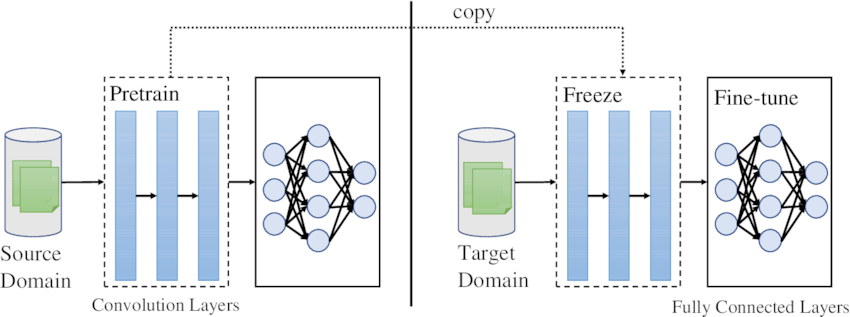
\includegraphics[width=0.8\textwidth]{transfer_learning_paradigm.png}
    \captionof{figure}{Mô hình Học Chuyển giao trong NLP: Một mô hình được huấn luyện trước trên dữ liệu lớn, sau đó được tinh chỉnh trên một tác vụ cụ thể.}
    \label{fig:transfer_learning_paradigm}
\end{center}

\textbf{Tại sao Học Chuyển giao lại hiệu quả?}
\begin{itemize}
    \item \textbf{Tiết kiệm tài nguyên:} Chúng ta không cần phải huấn luyện một mô hình khổng lồ từ đầu cho mỗi tác vụ. Chúng ta tận dụng lại kiến thức đã được học từ quá trình pre-training tốn kém.
    \item \textbf{Cải thiện hiệu năng:} Các biểu diễn ngôn ngữ tổng quát học được từ dữ liệu lớn cung cấp một điểm khởi đầu tốt hơn nhiều so với việc khởi tạo trọng số ngẫu nhiên, giúp mô hình hội tụ nhanh hơn và đạt độ chính xác cao hơn, đặc biệt khi dữ liệu cho tác vụ cụ thể là có hạn.
    \item \textbf{Dân chủ hóa AI:} Cho phép các nhà phát triển và nhà nghiên cứu không có tài nguyên tính toán khổng lồ vẫn có thể xây dựng các ứng dụng NLP state-of-the-art bằng cách tinh chỉnh các mô hình đã được huấn luyện trước.
\end{itemize}

\subsection{Tinh chỉnh Toàn bộ (Full Fine-tuning)}
\label{ssec:full_finetuning}

Đây là phương pháp tinh chỉnh kinh điển và trực quan nhất.

\subsubsection{Cơ chế hoạt động}
\begin{itemize}
    \item \textbf{Bước 1: Tải mô hình đã huấn luyện trước.} Tải toàn bộ kiến trúc và trọng số của một mô hình như BERT hoặc RoBERTa.
    \item \textbf{Bước 2: Thay thế "đầu" của mô hình.} Mô hình gốc thường có một "đầu" (head) được thiết kế cho tác vụ pre-training (ví dụ, đầu MLM). Chúng ta sẽ loại bỏ cái đầu này và thay thế nó bằng một "đầu" mới, phù hợp với tác vụ hạ nguồn của mình.
        \begin{itemize}
            \item \textbf{Ví dụ (Phân loại câu):} Thêm một lớp tuyến tính (linear layer) đơn giản với một lớp softmax lên trên vector biểu diễn của token `[CLS]`. Số nơ-ron đầu ra của lớp này bằng số lớp cần phân loại.
            \item \textbf{Ví dụ (Gán nhãn chuỗi - NER):} Thêm một lớp tuyến tính lên trên vector biểu diễn của \textit{mỗi} token trong chuỗi.
        \end{itemize}
    \item \textbf{Bước 3: Huấn luyện trên dữ liệu của tác vụ mới.} Toàn bộ mô hình (cả phần thân đã được huấn luyện trước và cái đầu mới) được huấn luyện tiếp trên bộ dữ liệu gán nhãn của tác vụ mục tiêu.
    \item \textbf{Cập nhật trọng số:} Trong quá trình này, \textbf{tất cả các trọng số của mô hình}, từ lớp embedding dưới cùng đến lớp phân loại trên cùng, đều được cập nhật thông qua thuật toán lan truyền ngược để tối thiểu hóa hàm mất mát trên tác vụ mới.
\end{itemize}
Điều quan trọng là việc huấn luyện ở giai đoạn này thường sử dụng một \textbf{tốc độ học (learning rate) rất nhỏ}. Lý do là vì các trọng số đã được huấn luyện trước đã ở một điểm "khá tốt". Chúng ta chỉ muốn "tinh chỉnh" chúng một chút để thích ứng với dữ liệu mới, chứ không muốn phá vỡ các kiến thức quý giá đã học được bằng các bước cập nhật quá lớn.

\subsubsection{Chiến lược Tinh chỉnh Nâng cao}
Trong thực tế, việc tinh chỉnh không chỉ đơn giản là chạy lại quá trình huấn luyện. Có một số chiến lược để cải thiện hiệu quả:
\paragraph{Huấn luyện theo lớp phân biệt (Discriminative Layer-wise Training)}
\begin{itemize}
    \item \textbf{Trực giác:} Các lớp khác nhau của một mô hình học sâu học các loại đặc trưng khác nhau. Các lớp dưới cùng (gần input) học các đặc trưng rất chung (như cú pháp cơ bản), trong khi các lớp trên cùng học các đặc trưng trừu tượng và chuyên biệt hơn.
    \item \textbf{Chiến lược:} Khi tinh chỉnh, chúng ta nên cập nhật các lớp trên cùng nhiều hơn và các lớp dưới cùng ít hơn. Điều này được thực hiện bằng cách áp dụng các \textbf{tốc độ học khác nhau cho các lớp khác nhau}. Ví dụ, lớp phân loại mới có thể có learning rate là $10^{-3}$, các lớp Transformer trên cùng là $10^{-4}$, và các lớp Transformer dưới cùng là $10^{-5}$.
\end{itemize}

\paragraph{Rã đông Dần dần (Gradual Unfreezing)}
\begin{itemize}
    \item \textbf{Trực giác:} Để tránh "quên thảm khốc" (catastrophic forgetting) - nơi mô hình nhanh chóng quên đi kiến thức đã học trong quá trình pre-training - chúng ta nên giới thiệu dữ liệu mới một cách từ từ.
    \item \textbf{Chiến lược:}
        \begin{enumerate}
            \item Ban đầu, "đóng băng" (freeze) toàn bộ các lớp đã được huấn luyện trước và chỉ huấn luyện cái đầu phân loại mới trong một vài epoch.
            \item Sau đó, "rã đông" (unfreeze) lớp Transformer trên cùng và huấn luyện cả nó và cái đầu mới.
            \item Tiếp tục quá trình này, rã đông dần dần từng lớp từ trên xuống dưới, cho đến khi toàn bộ mô hình được huấn luyện.
        \end{enumerate}
\end{itemize}

\subsubsection{Ưu và Nhược điểm của Tinh chỉnh Toàn bộ}
\begin{tcolorbox}[
    title=Đánh giá Tinh chỉnh Toàn bộ (Full Fine-tuning),
    colback=blue!5!white, colframe=blue!75!black, fonttitle=\bfseries
]
\textbf{Ưu điểm:}
\begin{itemize}
    \item \textbf{Hiệu năng cao nhất:} Thường mang lại độ chính xác tốt nhất vì toàn bộ mô hình được tối ưu hóa một cách trọn vẹn cho tác vụ mục tiêu.
    \item \textbf{Tương đối đơn giản:} Là một phương pháp đã được thiết lập rõ ràng và dễ triển khai.
\end{itemize}
\textbf{Nhược điểm:}
\begin{itemize}
    \item \textbf{Cực kỳ tốn kém về tài nguyên:} Thách thức lớn nhất trong kỷ nguyên LLM. Nếu bạn có 10 tác vụ khác nhau, bạn phải lưu trữ \textbf{10 bản sao đầy đủ} của mô hình khổng lồ đã được tinh chỉnh, mỗi bản sao có thể nặng hàng trăm gigabyte.
    \item \textbf{Dễ bị "quên thảm khốc":} Nếu dữ liệu tinh chỉnh quá khác biệt so với dữ liệu pre-training, mô hình có thể mất đi các khả năng tổng quát của nó.
    \item \textbf{Rủi ro về bảo mật và ổn định:} Việc cập nhật toàn bộ trọng số có thể gây ra các hành vi không mong muốn.
\end{itemize}
\end{tcolorbox}

Những nhược điểm này, đặc biệt là về chi phí lưu trữ và tính toán, đã trở nên cực kỳ rõ rệt với sự bùng nổ của các mô hình hàng tỷ tham số. Điều này đã thúc đẩy mạnh mẽ sự phát triển của một hướng tiếp cận mới, hiệu quả hơn nhiều: \textbf{Kỹ thuật Tinh chỉnh Hiệu quả Tham số (Parameter-Efficient Fine-Tuning - PEFT)}, mà chúng ta sẽ khám phá chi tiết trong mục tiếp theo.